\hypertarget{a00020}{\subsection{Com\-Objects.\-Com\-Client\-Leave Klassenreferenz}
\label{a00020}\index{Com\-Objects.\-Com\-Client\-Leave@{Com\-Objects.\-Com\-Client\-Leave}}
}
Klassendiagramm für Com\-Objects.\-Com\-Client\-Leave\-:\begin{figure}[H]
\begin{center}
\leavevmode
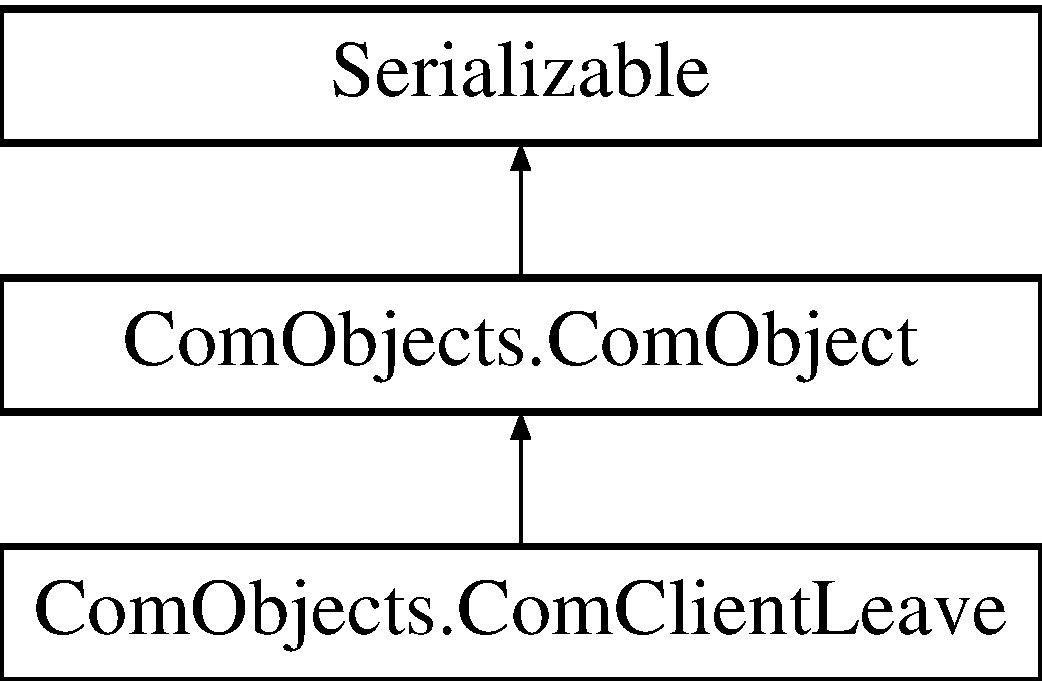
\includegraphics[height=3.000000cm]{a00020}
\end{center}
\end{figure}


\subsubsection{Ausführliche Beschreibung}
Sie wird zur Benachrichtigung gesendet, wenn ein Spieler ins nächste Fenster möchte und aus dem alten entfernt werden soll. 